\chapter{Rotatie- en vibratiespectroscopie}\label{ch:b3:rovibrational-spectroscopy}

Op een hoge, droge hoogvlakte richten tientallen radioantennes zich op een
donkere wolk tussen de sterren. Tussen de frequenties die ze opvangen zit
er een van
\qty{115.271}{GHz}: koolstofmonoxidemoleculen van enkele kelvin die van hun
eerste rotatieniveau naar het laagste overgaan. Uit dat ene getal haalt
een chemicus de lengte van de binding C--O tot op een fractie van een
picometer; uit de sterkte van de volgende lijnen de temperatuur van de
wolk. De rotaties en vibraties van moleculen zijn het onderwerp van dit
hoofdstuk: hun niveaus, uit de rotor en de oscillator van
\cref{ch:b3:quantum-model-systems}; de selectieregels, uit
\cref{ch:b3:group-theory-applied}; en wat spectra meten ---
bindingslengten, \omterm{def:b3:quantum-model-systems:oscillator}{krachtconstanten}, dissociatie-energieën.

\begin{recall}
\Cref{ch:b3:quantum-model-systems} gaf de \omterm{def:b3:quantum-model-systems:rotor}{starre rotor}, $E_J = J(J+1)\hbar^2/2I$
met \omterm{def:b3:quantum-model-systems:degenerate}{ontaardingsgraad} $2J + 1$, en de \omterm{def:b3:quantum-model-systems:oscillator}{harmonische oscillator}, $E_v = (v + \frac12)h\nu$,
voor een diatomisch molecuul met \omterm{def:b3:quantum-model-systems:oscillator}{gereduceerde massa} $\mu$.
\Cref{ch:b3:group-theory-applied} formuleerde de selectieregels voor
infrarood en Raman. Het deel van jaar~1 mat infraroodspectra in
golfgetallen en definieerde de polariseerbaarheid van een molecuul.
\end{recall}

\begin{omfigure}
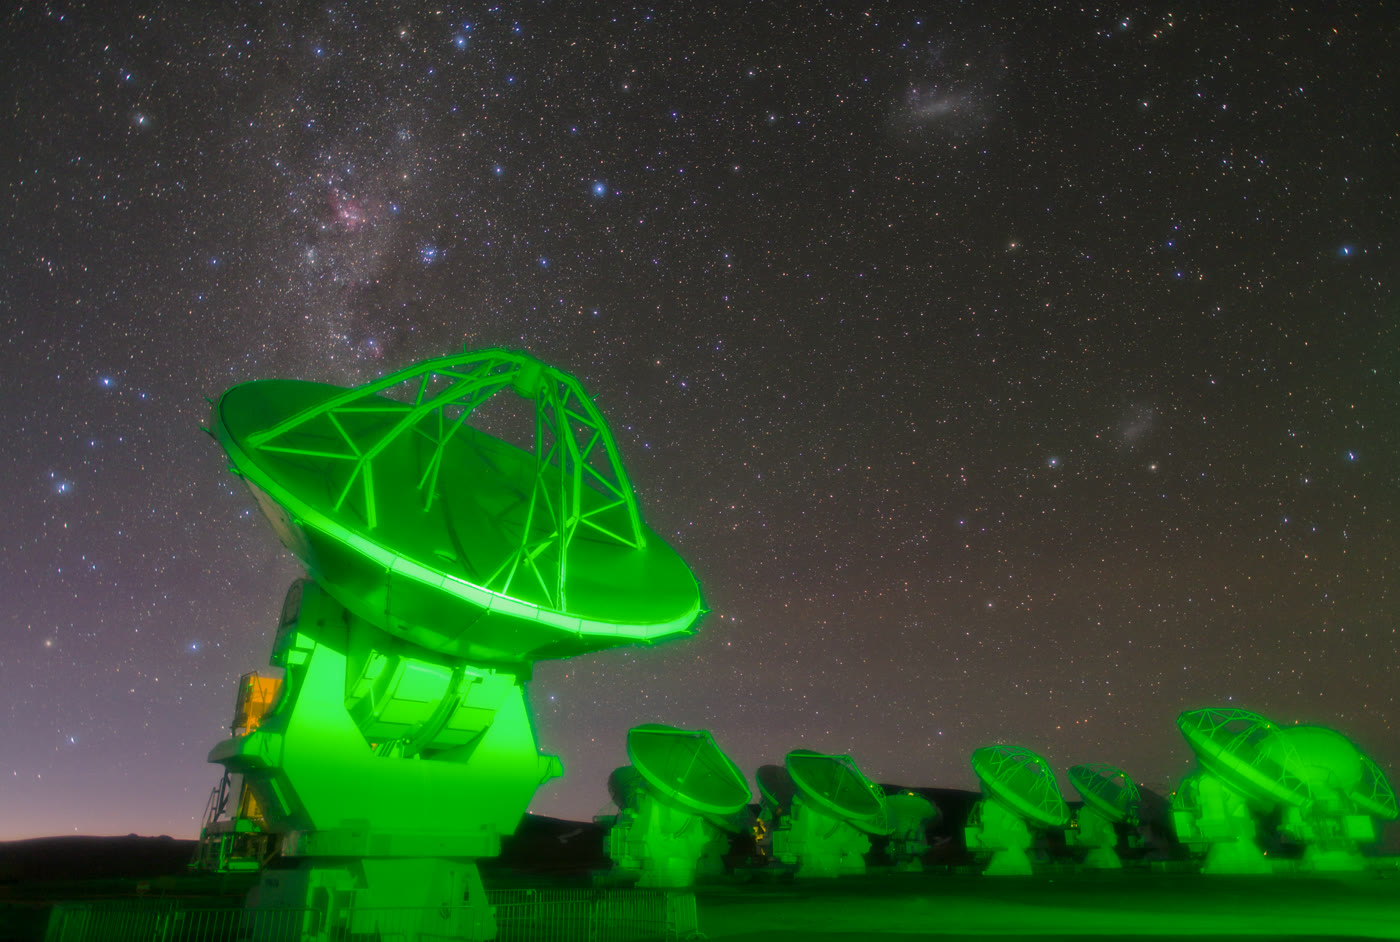
\includegraphics[width=0.7\linewidth]{images/book4/alma-antennas.jpg}

{\small Antennes van een radio-interferometer op een hoogvlakte: ze
registreren onder vele andere de rotatielijnen van koolstofmonoxide uit
interstellaire wolken. Foto ESO/B.~Tafreshi (twanight.org), CC BY 4.0.}
\end{omfigure}

\section{Rotatiespectra}

\begin{definition}[Rotatieconstante, isotopoloog]\label{def:b3:rovibrational-spectroscopy:rotational-constant}
De \emph{rotatieconstante}\index{rotatieconstante} van een lineair molecuul
is $B = h/(8\pi^2cI)$, in \unit{cm^{-1}} (of $B = h/8\pi^2I$ in hertz), zodat zijn
rotatieniveaus in golfgetallen $F(J) = BJ(J+1)$ zijn. Moleculen die alleen
verschillen in de isotopen van hun atomen, zijn
\emph{isotopologen}\index{isotopoloog}
(\ce{^{12}C^{16}O}, \ce{^{13}C^{16}O}); in de \omterm{def:b3:computational-chemistry:born-oppenheimer}{born-oppenheimerbenadering}
hebben ze dezelfde bindingslengten en \omterm{def:b3:quantum-model-systems:oscillator}{krachtconstanten}.
\end{definition}

\begin{definition}[Algemene en specifieke selectieregels]\label{def:b3:rovibrational-spectroscopy:selection}
Een \emph{algemene selectieregel}\index{algemene selectieregel} zegt welke
eigenschap een molecuul moet hebben om een bepaald soort spectrum
überhaupt te vertonen; een
\emph{specifieke selectieregel}\index{specifieke selectieregel} zegt welke
veranderingen van kwantumgetal toegestaan zijn.
\end{definition}

\begin{proposition}[Zuivere rotatiespectra]\label{prop:b3:rovibrational-spectroscopy:rotational-lines}
Een molecuul heeft alleen een zuiver rotatiespectrum (microgolfspectrum)
als het een permanent dipoolmoment heeft; voor een lineair molecuul is de
specifieke regel $\Delta J
= \pm1$. De absorptielijnen liggen bij
\[
\tilde\nu = F(J+1) - F(J) = 2B(J + 1), \qquad J = 0, 1, 2, \dots,
\]
op gelijke afstanden $2B$.
\end{proposition}

\begin{proof}
De wisselwerking met licht verloopt via het dipoolmoment: een molecuul
zonder permanente dipool heeft geen oscillerende dipool wanneer het
roteert. De regel $\Delta J
= \pm1$ volgt uit het nul zijn van $\int Y_{J'M'}^*\cos\theta\,Y_{JM}$ tenzij $J' = J
\pm 1$ (de dipoolcomponent langs $z$ transformeert als $Y_{1,0}$), hier
aangenomen.
Dan is $B(J+1)(J+2) - BJ(J+1) = 2B(J+1)$.
\end{proof}

\begin{method}[Bindingslengte uit een rotatielijn]\label{met:b3:rovibrational-spectroscopy:bond-length}
\begin{enumerate}
  \item Leid uit de lijn $J + 1 \leftarrow J$ met frequentie $\nu$ af dat $B =
        \nu/2(J+1)$ (in hertz).
  \item Bereken het traagheidsmoment $I = h/8\pi^2B$.
  \item Met de \omterm{def:b3:quantum-model-systems:oscillator}{gereduceerde massa} uit de isotoopmassa's is $r = \sqrt{I/\mu}$.
\end{enumerate}
\end{method}

\begin{example}[Koolstofmonoxide]\label{ex:b3:rovibrational-spectroscopy:co}
% ledger: rotl:CO.1-0, imass:O16
De lijn $J = 1 \leftarrow 0$ van \ce{^{12}C^{16}O} ligt bij \qty{115271.20}{MHz}:
$B = \qty{57635.6}{MHz} = \qty{1.92252}{cm^{-1}}$, $I = \qty{1.4560e-46}{kg.m^2}$.
Met $\mu = 12 \times 15.99491/27.99491 = \qty{6.85621}{u}$ is $r_0 = \qty{113.09}{pm}$.
Deze $r_0$ middelt de binding over haar nulpuntsvibratie en is iets langer
dan de evenwichtslengte $r_e$ (\cref{sec:b3:rovibrational-spectroscopy:real-bonds}).
\end{example}

\begin{definition}[Centrifugale distorsieconstante]\label{def:b3:rovibrational-spectroscopy:centrifugal}
Een roterende binding rekt uit; de niveaus worden $F(J) = BJ(J+1) - DJ^2(J+1)^2$,
waarin $D$ de \emph{centrifugale distorsieconstante}\index{centrifugale distorsieconstante}
is, en de lijnen $2B(J+1) - 4D(J+1)^3$ schuiven bij hoge $J$ langzaam naar
elkaar toe.
\end{definition}

\begin{proposition}[De sterkste lijn]\label{prop:b3:rovibrational-spectroscopy:jmax}
Als de lijnintensiteiten de bezetting van het lagere niveau volgen, $(2J+1)
\eu^{-hcBJ(J+1)/kT}$, ligt het sterkst bezette niveau bij ongeveer
\[
J_{\max} \approx \sqrt{\frac{kT}{2hcB}} - \frac12.
\]
\end{proposition}

\begin{proof}
Behandel $J$ als continu en differentieer: $\frac{\dd}{\dd J}[(2J+1)\eu^{-aJ(J+1)}]
= [2 - a(2J+1)^2]\eu^{-aJ(J+1)}$ met $a = hcB/kT$; dit is nul voor $(2J + 1)^2 =
2/a$.
\end{proof}

\begin{omfigure}
\begin{tikzpicture}
\begin{axis}[width=0.9\linewidth, height=4.8cm, xmin=0, xmax=70, ymin=0,
  ymax=1.12, ytick=\empty, axis x line=bottom, axis y line=left, ycomb,
  xlabel={golfgetal / cm$^{-1}$}, ylabel={relatieve intensiteit},
  tick label style={font=\small}, label style={font=\small}]
\addplot[omDef, very thick] table[x=nu, y=I] {figdata/out/bachelor-3-rotational-spectrum-co-30.dat};
\addplot[omThm, thick, xshift=1.2pt] table[x=nu, y=I] {figdata/out/bachelor-3-rotational-spectrum-co-300.dat};
\end{axis}
\end{tikzpicture}

{\small Het rotatieabsorptiespectrum van koolstofmonoxide, met lijnen op
afstanden $2B = \qty{3.845}{cm^{-1}}$ en intensiteiten gelijk genomen aan
de bezetting van het lagere niveau, bij \qty{30}{K} (blauw) en \qty{300}{K}
(rood, licht verschoven voor de zichtbaarheid), elke temperatuur
geschaald op haar sterkste lijn. Bij \qty{30}{K} is de sterkste lijn
$J = 3 \leftarrow 2$; bij \qty{300}{K} $J = 8 \leftarrow 7$.}
\end{omfigure}

\section{Vibraties van echte bindingen}\label{sec:b3:rovibrational-spectroscopy:real-bonds}

Een echte binding gehoorzaamt ver van het evenwicht niet aan de wet van
Hooke: ze wordt slapper wanneer ze uitgerekt wordt, en breekt.

\begin{definition}[Morsepotentiaal]\label{def:b3:rovibrational-spectroscopy:morse}
De \emph{morsepotentiaal}\index{morsepotentiaal} is $V(r) = D_e[1 -
\eu^{-\beta(r - r_e)}]^2$: harmonisch nabij $r_e$ (\omterm{def:b3:quantum-model-systems:oscillator}{krachtconstante} $2\beta^2D_e$), en
naderend tot de dissociatiegrens $D_e$ bij grote $r$.
\end{definition}

\begin{proposition}[Niveaus van de morseoscillator]\label{prop:b3:rovibrational-spectroscopy:morse-levels}
In golfgetallen zijn de vibratieniveaus van een morseoscillator
\[
G(v) = \tilde\omega_e(v + \tfrac12) - \tilde\omega_ex_e(v + \tfrac12)^2, \qquad
\tilde\omega_ex_e = \frac{\tilde\omega_e^2}{4D_e},
\]
een ladder waarvan de sporten dichter bij elkaar komen en die eindigt bij $v_{\max} = \lfloor\tilde\omega_e/
2\tilde\omega_ex_e - \frac12\rfloor$.
\end{proposition}
\admitted

De oplossing van de morsevergelijking hoort thuis in meer gevorderde
cursussen; de niveaus worden numeriek gecontroleerd in de figuurgegevens
van dit hoofdstuk.

\begin{definition}[Anharmoniciteitsconstante, fundamentele overgang, boventoon, hete band]\label{def:b3:rovibrational-spectroscopy:anharmonic}
$\tilde\omega_ex_e$ is de \emph{anharmoniciteitsconstante}\index{anharmoniciteitsconstante}.
De \emph{fundamentele overgang}\index{fundamentele overgang}
is $v = 1 \leftarrow 0$; een \emph{boventoon}\index{boventoon} is $v = n \leftarrow 0$
met $n \ge 2$, zwak omdat de algemene regel $\Delta v = \pm1$ van de
\omterm{def:b3:quantum-model-systems:oscillator}{harmonische oscillator} maar licht doorbroken wordt; een
\emph{hete band}\index{hete band} vertrekt
van een aangeslagen niveau, $v = 2 \leftarrow 1$, en groeit met de temperatuur.
\end{definition}

\begin{definition}[Spectroscopische dissociatie-energie]\label{def:b3:rovibrational-spectroscopy:dissociation}
De \emph{spectroscopische dissociatie-energie}\index{spectroscopische dissociatie-energie}
van een molecuul is de diepte van zijn potentiaal, $D_e$, gemeten vanaf het
minimum, of $D_0 = D_e - G(0)$, gemeten vanaf het laagste niveau --- per
molecuul bij \qty{0}{K}, in tegenstelling tot de
bindingsdissociatie-enthalpie uit het deel van jaar~2, een molaire
enthalpie bij \qty{298}{K}.
\end{definition}

\begin{corollary}[$D_e$ en $D_0$ van een morseoscillator]\label{cor:b3:rovibrational-spectroscopy:de}
$D_e = \tilde\omega_e^2/4\tilde\omega_ex_e$ en $D_0 = D_e - (\frac12\tilde\omega_e -
\frac14\tilde\omega_ex_e)$.
\end{corollary}

\begin{proof}
De eerste is de betrekking uit de propositie; de tweede is $G(0)$.
\end{proof}

\begin{proposition}[Extrapolatie van Birge-Sponer]\label{prop:b3:rovibrational-spectroscopy:birge-sponer}
De afstanden $\Delta G(v + \frac12) = G(v+1) - G(v) = \tilde\omega_e - 2\tilde\omega_ex_e(v +
1)$ nemen lineair af met $v$; hun som tot ze nul worden, geeft $D_0$, de
oppervlakte onder de grafiek van $\Delta G$ tegen $v$.
\end{proposition}

\begin{proof}
Trek de twee uitdrukkingen voor $G$ van elkaar af. $D_0$ is de energie van
$v = 0$ tot de grens, de som van alle afstanden.
\end{proof}

\begin{example}[Waterstofchloride]\label{ex:b3:rovibrational-spectroscopy:hcl}
% ledger: diat:HCl.we, diat:HCl.wexe, janaf:H.dfH0, janaf:Cl.dfH0, janaf:HCl.dfH0
Voor \ce{H^{35}Cl} is $\tilde\omega_e = \qty{2990.95}{cm^{-1}}$ en $\tilde\omega_ex_e =
\qty{52.82}{cm^{-1}}$: de \omterm{def:b3:rovibrational-spectroscopy:anharmonic}{fundamentele overgang} ligt bij $\tilde\omega_e - 2\tilde\omega_ex_e =
\qty{2885.3}{cm^{-1}}$ en de eerste \omterm{def:b3:rovibrational-spectroscopy:anharmonic}{boventoon} bij $2\tilde\omega_e - 6\tilde\omega_ex_e =
\qty{5665.0}{cm^{-1}}$, iets minder dan het dubbele van de fundamentele.
Het morsemodel voorspelt $D_e = \qty{42342}{cm^{-1}}$ en $D_0 = \qty{40860}{cm^{-1}}$; de echte $D_0$,
uit de vormingsenthalpieën van H, Cl en HCl bij \qty{0}{K}, is
\qty{35760}{cm^{-1}} (\qty{4.43}{eV}). De echte potentiaal vlakt sneller af
dan een morsekromme die op de bodem aangepast is: extrapolaties van
Birge-Sponer vanuit de laagste niveaus overschatten
dissociatie-energieën.
\end{example}

\begin{omfigure}
\begin{tikzpicture}
\begin{axis}[name=morse, width=0.55\linewidth, height=6cm, xmin=0.8, xmax=4.0,
  ymin=0, ymax=48000, axis lines=left, xlabel={$r$ / \AA}, ylabel={$V$ / cm$^{-1}$},
  unbounded coords=jump, scaled y ticks=false, ytick={0,10000,20000,30000,40000},
  tick label style={font=\small}, label style={font=\small}]
\addplot[black, thick] table[x=r, y=V] {figdata/out/bachelor-3-morse-levels.dat};
\addplot[gray, dashed] table[x=r, y=harm] {figdata/out/bachelor-3-morse-levels.dat};
\addplot[omDef] table[x=r, y=E] {figdata/out/bachelor-3-morse-levels-levels.dat};
\draw[<->, omThm] (axis cs:3.7,0) -- (axis cs:3.7,42342) node[pos=0.5, left, font=\small] {$D_e$};
\draw[dashed, omThm] (axis cs:1.2,42342) -- (axis cs:4.0,42342);
\end{axis}
\begin{axis}[at={(morse.east)}, anchor=west, xshift=1.6cm, width=0.4\linewidth,
  height=5cm, xmin=0, xmax=28, ymin=0, ymax=3100, axis lines=left,
  xlabel={$v$}, ylabel={$\Delta G(v + \frac12)$ / cm$^{-1}$},
  tick label style={font=\small}, label style={font=\small}]
\addplot[omDef, only marks, mark size=1.2pt] table[x=v, y=dG] {figdata/out/bachelor-3-morse-levels-bs.dat};
\addplot[omDef!40, fill=omDef!12, draw=none] table[x=v, y=dG] {figdata/out/bachelor-3-morse-levels-bs.dat} \closedcycle;
\end{axis}
\end{tikzpicture}

{\small Links: de \omterm{def:b3:rovibrational-spectroscopy:morse}{morsepotentiaal} van \ce{HCl}, opgebouwd uit zijn
spectroscopische constanten (doorgetrokken), de harmonische parabool met
dezelfde kromming (gestreept), en elk derde vibratieniveau, getekend
tussen zijn keerpunten; de niveaus komen dichter bij elkaar naar $D_e$
toe. Rechts: de grafiek van Birge-Sponer van de afstanden; de gearceerde
oppervlakte is $D_0$.}
\end{omfigure}

\section{Rotatie-vibratiebanden}

Een vibratieovergang van een gas gaat gepaard met rotatieveranderingen, $\Delta
J = \pm1$ voor een diatomisch molecuul in een toestand ${}^1\Sigma$.

\begin{definition}[P-, Q- en R-tak, bandoorsprong]\label{def:b3:rovibrational-spectroscopy:branches}
In een rotatie-vibratieband vormen de lijnen met $\Delta J = -1$ de
\emph{P-tak}\index{P-tak}, die met $\Delta J = +1$ de \emph{R-tak}\index{R-tak},
en die met $\Delta J = 0$, als ze toegestaan zijn, de \emph{Q-tak}\index{Q-tak}.
De \emph{bandoorsprong}\index{bandoorsprong} $\tilde\nu_0$ is het
vibratie-energieverschil zonder rotatie.
\end{definition}

\begin{theorem}[Combinatieverschillen]\label{thm:b3:rovibrational-spectroscopy:combination-differences}
Met de \omterm{def:b3:rovibrational-spectroscopy:rotational-constant}{rotatieconstanten} $B_0$ en $B_1$ in het lagere en het hogere
vibratieniveau is $R(J) = \tilde\nu_0 + B_1(J+1)(J+2) - B_0J(J+1)$ en $P(J) = \tilde\nu_0 +
B_1(J-1)J - B_0J(J+1)$, en
\[
R(J - 1) - P(J + 1) = 4B_0(J + \tfrac12), \qquad R(J) - P(J) = 4B_1(J + \tfrac12).
\]
\end{theorem}

\begin{proof}
De eerste twee volgen uit $E = G(v) + B_vJ(J+1)$ voor beide niveaus. $R(J - 1)$ en
$P(J + 1)$ eindigen op hetzelfde hogere niveau $J$, vanuit de lagere
niveaus $J - 1$ en $J + 1$:
hun verschil is $B_0[(J+1)(J+2) - (J-1)J] = B_0(4J + 2)$. Op dezelfde manier vertrekken $R(J)$ en
$P(J)$ vanuit hetzelfde lagere niveau en eindigen ze op $J + 1$ en $J - 1$.
\end{proof}

\begin{method}[Een rotatie-vibratieband analyseren]\label{met:b3:rovibrational-spectroscopy:combination}
\begin{enumerate}
  \item Zoek de opening: voor een diatomisch molecuul ${}^1\Sigma$ is er
        geen \omterm{def:b3:rovibrational-spectroscopy:branches}{Q-tak}, en
        $\tilde\nu_0$ ligt in de opening, tussen $R(0)$ en $P(1)$.
  \item Nummer de lijnen vanaf de opening naar buiten: $R(0), R(1), \dots$ en $P(1),
        P(2), \dots$.
  \item Gebruik de combinatieverschillen om $B_0$ en $B_1$ afzonderlijk te
        vinden, en daarna $\alpha_e = B_0 - B_1$ en $B_e = B_0 + \frac12\alpha_e$.
\end{enumerate}
\end{method}

\begin{omfigure}
\begin{tikzpicture}
\begin{axis}[width=0.92\linewidth, height=5cm, xmin=2650, xmax=3080, ymin=0,
  ymax=1.15, ytick=\empty, axis x line=bottom, axis y line=left,
  xlabel={golfgetal / cm$^{-1}$}, ylabel={absorbantie (relatief)},
  tick label style={font=\small}, label style={font=\small}]
\addplot[omDef, thin] table[x=nu, y=A] {figdata/out/bachelor-3-rovib-band.dat};
\node[font=\small] at (axis cs:2780,1.06) {P-tak};
\node[font=\small] at (axis cs:2985,1.06) {R-tak};
\draw[->, gray] (axis cs:2885.3,0.45) -- (axis cs:2885.3,0.05);
\node[font=\small, gray, anchor=south] at (axis cs:2885.3,0.45) {$\tilde\nu_0$};
\end{axis}
\end{tikzpicture}

{\small De fundamentele band van gasvormig \ce{HCl} bij \qty{300}{K},
berekend uit zijn spectroscopische constanten: P- en \omterm{def:b3:rovibrational-spectroscopy:branches}{R-tak} aan weerszijden
van de opening bij de \omterm{def:b3:rovibrational-spectroscopy:branches}{bandoorsprong}. Elke lijn is een doublet,
\ce{H^{35}Cl} en het zwakkere, iets lager liggende \ce{H^{37}Cl}
(natuurlijke abundanties 76\,\% en 24\,\%). De R-lijnen komen dichter bij
elkaar, de P-lijnen spreiden uit, omdat $B_1 < B_0$.}
\end{omfigure}

\begin{example}[De constanten van \ce{HCl} uit zijn band]\label{ex:b3:rovibrational-spectroscopy:analysis}
% ledger: diat:HCl.Be, diat:HCl.ae
Met $R(0) = \qty{2905.58}{cm^{-1}}$ en $P(2) = \qty{2842.94}{cm^{-1}}$ vindt men
$6B_0 = \qty{62.64}{cm^{-1}}$, dus $B_0 = \qty{10.440}{cm^{-1}}$. Met $R(1) = 2925.23$ en $P(1) =
\qty{2864.43}{cm^{-1}}$ is $B_1 = \qty{10.133}{cm^{-1}}$. Dus $\alpha_e = \qty{0.307}{cm^{-1}}$
en $B_e = \qty{10.593}{cm^{-1}}$, de waarden waaruit de band werd opgebouwd:
de methode vindt ze exact terug.
\end{example}

\section{Ramanspectroscopie}

\begin{definition}[Raman- en rayleighverstrooiing]\label{def:b3:rovibrational-spectroscopy:raman}
Wanneer licht met frequentie $\nu_0$ door een monster gaat, behoudt het
meeste verstrooide licht de frequentie $\nu_0$:
\emph{rayleighverstrooiing}\index{rayleighverstrooiing}.
Een kleine fractie is verschoven met de rotatie- of vibratiefrequenties
van de moleculen: \emph{ramanverstrooiing}\index{ramanverstrooiing}.
Lijnen bij lagere frequentie zijn \emph{stokeslijnen}\index{stokeslijn} (het
molecuul heeft energie gewonnen), lijnen bij hogere frequentie
\emph{anti-stokeslijnen}\index{anti-stokeslijn} (het heeft energie verloren).
\end{definition}

\begin{proposition}[Klassieke oorsprong van het ramaneffect]\label{prop:b3:rovibrational-spectroscopy:raman-classical}
Als de polariseerbaarheid van een molecuul dat met $\nu_{\mathrm{vib}}$ trilt,
varieert als $\alpha = \alpha_0 + \alpha_1\cos(2\pi\nu_{\mathrm{vib}}t)$, dan
oscilleert de dipool die geïnduceerd wordt door een
veld $E_0\cos(2\pi\nu_0t)$ met $\nu_0$ en met $\nu_0 \pm \nu_{\mathrm{vib}}$.
Een vibratie is alleen \omterm{def:b3:group-theory-applied:activity}{Raman-actief} als ze de polariseerbaarheid verandert.
\end{proposition}

\begin{proof}
$\mu = \alpha E = \alpha_0E_0\cos(2\pi\nu_0t) + \frac12\alpha_1E_0[\cos2\pi(\nu_0 +
\nu_{\mathrm{vib}})t + \cos2\pi(\nu_0 - \nu_{\mathrm{vib}})t]$, want $\cos a\cos b =
\frac12[\cos(a+b) + \cos(a-b)]$. Elke oscillerende dipool straalt uit met
zijn eigen frequentie; zonder $\alpha_1$ blijft alleen de rayleighterm over.
\end{proof}

\begin{proposition}[Rotatieramanlijnen]\label{prop:b3:rovibrational-spectroscopy:rotational-raman}
Een lineair molecuul met een anisotrope polariseerbaarheid vertoont
rotatieramanlijnen met $\Delta J = \pm2$, verschoven ten opzichte van de
excitatielijn met
\[
|\Delta\tilde\nu| = F(J+2) - F(J) = 4B(J + \tfrac32) = 6B, 10B, 14B, \dots
\]
--- de eerste lijn bij $6B$, daarna een tussenafstand van $4B$.
\end{proposition}

\begin{proof}
De polariseerbaarheidsellipsoïde van een roterend lineair molecuul keert
twee keer per omwenteling terug naar dezelfde oriëntatie, zodat ze de
verstrooiing moduleert met het dubbele van de rotatiefrequentie: $\Delta J = \pm2$ (de
kwantumregel, hier aangenomen). Dan is
$B(J+2)(J+3) - BJ(J+1) = B(4J + 6)$.
\end{proof}

\begin{example}[Stikstof, gezien door Raman]\label{ex:b3:rovibrational-spectroscopy:n2}
% ledger: diat:N2.Be, diat:N2.ae
\ce{N2} heeft geen dipool en geen infrarood- of microgolfspectrum, maar
zijn polariseerbaarheid is anisotroop: zijn rotatieramanlijnen beginnen
op $6B_0 =
\qty{11.94}{cm^{-1}}$ van de excitatielijn en liggen \qty{7.96}{cm^{-1}}
uit elkaar. Hun intensiteiten wisselen 2:1 af tussen even en oneven $J$:
de twee \ce{^{14}N}-kernen zijn identiek, en de kernspinstatistiek
(\cref{ch:b3:statistical-thermo-applied}) geeft niveaus met even $J$ het
dubbele gewicht van oneven niveaus.
\end{example}

\begin{omfigure}
\begin{tikzpicture}
\begin{axis}[name=r, width=0.55\linewidth, height=4.6cm, xmin=-110, xmax=110,
  ymin=0, ymax=1.1, ytick=\empty, axis x line=bottom, axis y line=left, ycomb,
  xlabel={ramanverschuiving / cm$^{-1}$}, tick label style={font=\small}, label style={font=\small},
  title={\small \ce{N2}, rotatieraman, \qty{300}{K}}]
\addplot[omDef, thick] table[x=shift, y=I] {figdata/out/bachelor-3-rotational-spectrum-n2-raman.dat};
\draw[gray, thick] (axis cs:0,0) -- (axis cs:0,1.05);
\end{axis}
\begin{scope}[xshift=0.6\linewidth, font=\small]
  \draw[omstate] (0,0) -- (2.4,0) node[right] {$v = 0$};
  \draw[omstate] (0,1.0) -- (2.4,1.0) node[right] {$v = 1$};
  \draw[omvib, densely dashed] (0,3.2) -- (2.4,3.2) node[right] {virtueel};
  \draw[omabs] (0.3,0) -- (0.3,3.18);
  \draw[omfluo] (0.5,3.18) -- (0.5,0.02);
  \node[font=\scriptsize, omThm, anchor=east] at (0.22,1.6) {Rayleigh};
  \draw[omabs] (1.3,0) -- (1.3,3.18);
  \draw[omphos] (1.5,3.18) -- (1.5,1.02) node[pos=0.4, right, font=\scriptsize] {Stokes};
\end{scope}
\end{tikzpicture}

{\small Links: het rotatieramanspectrum van stikstof, berekend bij
\qty{300}{K}: \omterm{def:b3:rovibrational-spectroscopy:raman}{stokeslijnen} bij positieve verschuivingen (rechts),
\omterm{def:b3:rovibrational-spectroscopy:raman}{anti-stokeslijnen} bij negatieve verschuivingen (links, iets zwakker), met
de afwisseling 2:1 van de intensiteiten; de grijze lijn bij nul geeft de
veel sterkere rayleighlijn aan. Rechts: energieschema van rayleigh- en
stokesverstrooiing via een virtueel niveau (geen echte toestand van het
molecuul).}
\end{omfigure}

\section{Meeratomige moleculen}

\begin{definition}[Soorten rotoren]\label{def:b3:rovibrational-spectroscopy:rotor-types}
Een molecuul met drie gelijke hoofdtraagheidsmomenten is een
\emph{sferische tol}\index{sferische tol} (\ce{CH4}, \ce{SF6}); met twee
gelijke een
\emph{symmetrische tol}\index{symmetrische tol} (\ce{NH3}, \ce{CHCl3}, \ce{C6H6});
met alle drie verschillend een \emph{asymmetrische tol}\index{asymmetrische tol}
(\ce{H2O}, de meeste moleculen); lineaire moleculen hebben één moment nul.
\end{definition}

Een \omterm{def:b3:rovibrational-spectroscopy:rotor-types}{sferische tol} heeft geen dipool en geen rotatiespectrum; een
\omterm{def:b3:rovibrational-spectroscopy:rotor-types}{symmetrische tol} heeft de niveaus $BJ(J+1) + (A - B)K^2$, waarin $K$ het
impulsmoment om zijn as telt,
en lijnen die nog steeds bij $2B(J+1)$ vallen, omdat $\Delta K = 0$; een
\omterm{def:b3:rovibrational-spectroscopy:rotor-types}{asymmetrische tol} heeft een onregelmatig spectrum, dat met de computer
aangepast wordt. De vibraties van meeratomige moleculen zijn hun
\omterm{def:b3:group-theory-applied:normal-mode}{normaaltrillingen}, benoemd en geselecteerd volgens
\cref{ch:b3:group-theory-applied}: het infraroodspectrum toont de
trillingen die transformeren als $x$, $y$, $z$, elk met zijn eigen
rotatiestructuur.

\begin{inthelab}[Een gascel in een infraroodspectrometer]
Gasvormig \ce{HCl} wordt binnengelaten in een cel van \qty{10}{cm} met
vensters die doorzichtig zijn in het infrarood, in een
fouriertransformatiespectrometer. Bij een resolutie van \qty{1}{cm^{-1}}
verschijnen de P- en R-takken als enkelvoudige lijnen; bij \qty{0.25}{cm^{-1}} splitst elke
lijn op in haar doublet \ce{H^{35}Cl}/\ce{H^{37}Cl}, met \qty{2}{cm^{-1}}
tussenafstand. Waterstofchloride is giftig en corrosief: de cel wordt
gevuld aan een vacuümlijn in een zuurkast.
\end{inthelab}

\begin{safety}{\ghs[0.8cm]{GHS04}\ghs[0.8cm]{GHS05}\ghs[0.8cm]{GHS06}}
Waterstofchloridegas: een gas onder druk, corrosief voor huid, ogen en
luchtwegen, giftig bij inademing. Alleen te hanteren in een gesloten
opstelling of in een zuurkast.
\end{safety}

\begin{history}[Raman, 1928]
In 1928 namen C. V. Raman en K. S. Krishnan, in zonlicht dat door een
violet filter gefilterd en door vloeistoffen verstrooid werd, een zwak licht
van een andere kleur waar, dat met een gekruist groen filter geïsoleerd
kon worden. Raman ontving de Nobelprijs voor de Natuurkunde van 1930;
laserbronnen maakten vijftig jaar later van zijn effect een
routinematige analysetechniek.
\end{history}

\section{Oefeningen}

\begin{exercise}[$\star$]\label{exo:b3:rovibrational-spectroscopy:1}
% ledger: imass:O16
Bereken uit $B_0 = \qty{1.9225}{cm^{-1}}$ voor \ce{^{12}C^{16}O} het
traagheidsmoment en de bindingslengte $r_0$.
\end{exercise}

\begin{exercise}[$\star$]\label{exo:b3:rovibrational-spectroscopy:2}
% ledger: diat:HCl.Be, diat:HCl.ae
Geef met $B_0 = \qty{10.440}{cm^{-1}}$ de posities van de eerste vier
lijnen van het rotatiespectrum van \ce{H^{35}Cl}, en de $J$ van de sterkste lijn bij
\qty{300}{K}.
\end{exercise}

\begin{exercise}[$\star$]\label{exo:b3:rovibrational-spectroscopy:3}
Welke van \ce{H2}, \ce{HCl}, \ce{N2}, \ce{CO2}, \ce{CH4}, \ce{SF6} en \ce{H2O} vertonen
een zuiver rotatieabsorptiespectrum? Een rotatieramanspectrum?
\end{exercise}

\begin{exercise}[$\star$]\label{exo:b3:rovibrational-spectroscopy:4}
% ledger: diat:HCl.we, diat:HCl.wexe
Welke fractie van de \ce{HCl}-moleculen bevindt zich in $v = 1$ bij 300 en
\qty{1000}{K} (\omterm{def:b3:rovibrational-spectroscopy:anharmonic}{fundamentele overgang} bij \qty{2885.3}{cm^{-1}})? Wanneer
wordt de \omterm{def:b3:rovibrational-spectroscopy:anharmonic}{hete band} zichtbaar?
\end{exercise}

\begin{exercise}[$\star\star$]\label{exo:b3:rovibrational-spectroscopy:5}
De \omterm{def:b3:rovibrational-spectroscopy:anharmonic}{fundamentele overgang} en de eerste \omterm{def:b3:rovibrational-spectroscopy:anharmonic}{boventoon} van \ce{H^{35}Cl} liggen
bij 2885.3 en
\qty{5665.0}{cm^{-1}}. Leid $\tilde\omega_e$ en $\tilde\omega_ex_e$ af.
\end{exercise}

\begin{exercise}[$\star\star$]\label{exo:b3:rovibrational-spectroscopy:6}
Bereken met de constanten van de vorige oefening $D_e$ en $D_0$ van het
morsemodel, en vergelijk met de echte $D_0 = \qty{35760}{cm^{-1}}$. Zet beide
waarden van $D_0$ om in \unit{kJ/mol}.
\end{exercise}

\begin{exercise}[$\star\star$]\label{exo:b3:rovibrational-spectroscopy:7}
Vier lijnen van de fundamentele band van \ce{H^{35}Cl} zijn $R(0) = 2905.58$, $R(1) = 2925.23$,
$P(1) = 2864.43$ en $P(2) = \qty{2842.94}{cm^{-1}}$. Bepaal $B_0$, $B_1$, $\alpha_e$ en
de \omterm{def:b3:rovibrational-spectroscopy:branches}{bandoorsprong}.
\end{exercise}

\begin{exercise}[$\star\star$]\label{exo:b3:rovibrational-spectroscopy:8}
% ledger: imass:H1, imass:H2, imass:Cl35
Voorspel $B_0$ en de \omterm{def:b3:rovibrational-spectroscopy:branches}{bandoorsprong} van \ce{D^{35}Cl} uit die van \ce{H^{35}Cl}, met
de \omterm{def:b3:quantum-model-systems:oscillator}{gereduceerde massa}'s ($\tilde\omega_e \propto \mu^{-1/2}$, $\tilde\omega_ex_e \propto
\mu^{-1}$, $B \propto \mu^{-1}$).
\end{exercise}

\begin{exercise}[$\star\star$]\label{exo:b3:rovibrational-spectroscopy:9}
% ledger: diat:N2.Be, diat:N2.ae
Voor \ce{N2} is $B_0 = \qty{1.9896}{cm^{-1}}$. Geef de verschuivingen van
de eerste drie stokesrotatieramanlijnen, en verklaar de afwisseling van
hun intensiteiten.
\end{exercise}

\begin{exercise}[$\star\star\star$]\label{exo:b3:rovibrational-spectroscopy:10}
% ledger: rotl:CO.1-0, rotl:CO.2-1, rotl:CO.3-2
De eerste drie rotatielijnen van \ce{^{12}C^{16}O} liggen bij 115271.2018,
230538.0000 en \qty{345795.9899}{MHz}. Toon aan dat een \omterm{def:b3:quantum-model-systems:rotor}{starre rotor} er
niet bij past, en bepaal $B$ en de \omterm{def:b3:rovibrational-spectroscopy:centrifugal}{centrifugale distorsieconstante} $D$.
\end{exercise}

\begin{exercise}[$\star\star\star$]\label{exo:b3:rovibrational-spectroscopy:11}
Toon aan dat de som van Birge-Sponer van de afstanden $\Delta G(v + \frac12)$ van een
morseoscillator, van $v = 0$ tot het laatste gebonden niveau, dicht bij
$D_e - G(0)$ ligt, en bereken de som voor \ce{HCl}.
\end{exercise}

\begin{exercise}[$\star\star\star$]\label{exo:b3:rovibrational-spectroscopy:12}
De \ce{^{16}O}-kern heeft spin nul, zodat de niveaus van \ce{^{16}O^{12}C^{16}O} met oneven
$J$ niet bestaan. Wat is de tussenafstand van zijn rotatieramanlijnen, en
de verschuiving van de eerste, uitgedrukt in $B$? Waarom heeft \ce{CO2} geen
microgolfspectrum?
\end{exercise}

\section{Probleem: luisteren naar een koude wolk}

\begin{problem}[{Weekendprobleem --- de bindingslengte van koolstofmonoxide
uit zijn eerste rotatielijn, de temperatuur van een interstellaire wolk,
de koolstof-13-isotopoloog, en de infraroodband}]
\label{pb:b3:rovibrational-spectroscopy:1}
% ledger: rotl:CO.1-0, rotl:CO.2-1, rotl:13CO.1-0, imass:O16, imass:C13, iso:C13, diat:CO.we, diat:CO.wexe, re:CO
Gegevens: lijnen van \ce{^{12}C^{16}O}: $J = 1 \leftarrow 0$ bij \qty{115.2712}{GHz} en $2
\leftarrow 1$ bij \qty{230.5380}{GHz}; lijn van \ce{^{13}C^{16}O}: $1 \leftarrow 0$ bij
\qty{110.2014}{GHz}; massa's \ce{^{12}C} 12 (exact), \ce{^{13}C} 13.00335,
\ce{^{16}O} \qty{15.99491}{u}; natuurlijke abundantie van \ce{^{13}C} 1.1\,\%; voor \ce{^{12}C^{16}O}
$\tilde\omega_e = \qty{2169.81}{cm^{-1}}$, $\tilde\omega_ex_e = \qty{13.288}{cm^{-1}}$, en de
evenwichtslengte $r_e = \qty{112.83}{pm}$. $h = \qty{6.62607e-34}{J.s}$, $u =
\qty{1.66054e-27}{kg}$, $c = \qty{2.99792e10}{cm/s}$, $hc/k = \qty{1.43878}{cm.K}$.

\medskip\noindent\textbf{Deel I --- De binding.}
\begin{enumerate}
  \item Bereken $B_0$ in hertz en in \unit{cm^{-1}}.
  \item Bereken de \omterm{def:b3:quantum-model-systems:oscillator}{gereduceerde massa} van \ce{^{12}C^{16}O} in kilogram.
  \item Bereken het traagheidsmoment.
  \item Leid $r_0$ af.
  \item Vergelijk met $r_e$. Waarom is $r_0$ langer?
  \item Voorspel de lijn $2 \leftarrow 1$ voor een \omterm{def:b3:quantum-model-systems:rotor}{starre rotor}.
        Becommentarieer de gemeten waarde.
\end{enumerate}

\medskip\noindent\textbf{Deel II --- De temperatuur van de wolk.}
\begin{enumerate}[resume]
  \item Geef de energieën, in \unit{cm^{-1}} en in kelvin ($E/k$), van de niveaus $J =
        0$, 1, 2.
  \item Schrijf de verhouding van de bezettingen $N_2/N_1$ bij temperatuur $T$.
  \item De waarnemingen geven $N_2/N_1 = 0.85$ (gegevens van het probleem).
        Bepaal $T$.
  \item Welk niveau is bij die temperatuur het sterkst bezet?
  \item Waarom kan zo'n wolk niet gezien worden in de infraroodvibratieband?
  \item Waarom is de lijn $1 \leftarrow 0$ de meest gebruikte tracer van koud gas?
\end{enumerate}

\medskip\noindent\textbf{Deel III --- De \omterm{def:b3:rovibrational-spectroscopy:rotational-constant}{isotopoloog}.}
\begin{enumerate}[resume]
  \item Bereken de \omterm{def:b3:quantum-model-systems:oscillator}{gereduceerde massa} van \ce{^{13}C^{16}O}.
  \item Voorspel zijn lijn $1 \leftarrow 0$ uit die van \ce{^{12}C^{16}O}.
  \item Vergelijk met de gemeten \qty{110.2014}{GHz}. Wat werd verwaarloosd?
  \item Als beide lijnen zwak en onverzadigd waren, welke verhouding van
        hun intensiteiten zouden de natuurlijke abundanties dan geven?
  \item De waargenomen verhouding is veel kleiner. Wat zegt dat over de lijn van
        \ce{^{12}C^{16}O}?
  \item Waarom worden beide \omterm{def:b3:rovibrational-spectroscopy:rotational-constant}{isotopologen} in de praktijk samen waargenomen?
\end{enumerate}

\medskip\noindent\textbf{Deel IV --- De vibratieband.}
\begin{enumerate}[resume]
  \item Bereken de \omterm{def:b3:rovibrational-spectroscopy:branches}{bandoorsprong} van de \omterm{def:b3:rovibrational-spectroscopy:anharmonic}{fundamentele overgang}, in
        \unit{cm^{-1}} en in micrometer.
  \item Bereken de eerste \omterm{def:b3:rovibrational-spectroscopy:anharmonic}{boventoon}.
  \item Bereken de \omterm{def:b3:quantum-model-systems:oscillator}{nulpuntsenergie}.
  \item Wat scheidt de eerste R- en P-lijn?
  \item Welk molecuul, \ce{^{12}C^{16}O} of \ce{^{13}C^{16}O}, heeft de laagste \omterm{def:b3:rovibrational-spectroscopy:branches}{bandoorsprong}?
  \item Formuleer het resultaat: de bindingslengte $r_0$ van
        koolstofmonoxide, verkregen uit één enkele radiolijn.
\end{enumerate}
\end{problem}
